\begin{frame}
    {Using ccECPs for solid state}
    \begin{itemize}
        \item If using gaussian basis sets, i.e. (PySCF), our potentials can be used as is, as shown previously.
        \item Using PBC, basis sets may need to be altered and/or reoptimized entirely. e.g. Diffuse functions can cause linear dependency issues, to fix add: \\
            {\color{darkblue}cell.drop\_exponent=0.1} in pySCF to the cell object
        \item If basis is problematic, contractions for occupied orbitals need to be tailored to the ECP. Often useful to use an ionized +1, +2 state to get contractions.\\
            Uncontracted primitives can come from existing solid-state basis sets. \\
            For inspiration, can use primitives from \url{http://www.crystal.unito.it/basis-sets.php} or \\
            \url{https://www.tcm.phy.cam.ac.uk/~mdt26/crystal.html}
    \end{itemize}
\end{frame}

\subsection{KB Transformation}
\begin{frame}
    \begin{columns}
        \begin{column}
            {0.4\textwidth}
            \centering
            {\color{ForestGreen}Semi-local potential}\\
            $\hat{V}_{\rm SL} = \sum\limits_{\ell m}  | \ell m\rangle V_\ell(r) \langle\ell m|$
        \end{column}
        \begin{column}
            {0.6\textwidth}
            \centering
            {\color{ForestGreen}KB potential}\\
            $\hat{V}_{\rm KB} = V_{\rm local}(r) + \sum\limits_{\ell m} \frac{| \phi_{\ell m}^{\rm PS} \delta V_\ell \rangle \langle \delta V_\ell \phi_{\ell m}^{\rm PS}|}{\langle \phi_{\ell m}^{\rm PS} |\delta V_\ell | \phi_{\ell m}^{\rm PS}\rangle} $
        \end{column}
    \end{columns}
    \bigskip
    \begin{itemize}
        \item[] {\color{NavyBlue} Ghost States:} Low energy states that have the wrong number of nodes. Can cause unphysical energies, difficulty, optimizing wave functions, unstable DMC, etc. (see Drummond, Trail, \& Needs, PRB {\bf 94}, 165170 (2016)).
        \item[] {\color{NavyBlue} Transferability:} Ability of a potential to perform the same as the reference. 
    \end{itemize}
    \bigskip

    We take our semi-local ccECPs to be an accurate representation of the AE Hamiltonian. Therefore, we need the KB version to be transferable with respect to the semi-local potential.

\end{frame}

\begin{frame}
    OPIUM is a norm-conserving pseudopotential generation tool to develop pseudopotentials for plane-wave codes like QE.\\
    \bigskip
    A modified version that can input gaussian parameterized semi-local potentials (ccECPs, Stuttgart, BFD, etc) has been used to generate the UPF files, and included some information about ghost states, transferability, recommended plane-wave cutoffs, in the .rpt file.
\end{frame}

\begin{frame}
    \begin{columns}
        \begin{column}
            {0.3\textwidth}
		    \begin{tikzpicture}
                \node [anchor=west] (water) at (0.25,0.35) {};
		        \begin{scope}[xshift=1.5cm]
		            \node[anchor=south west,inner sep=0] (image) at (0,0) {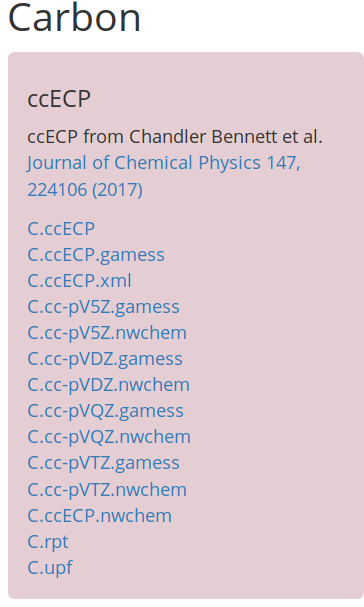
\includegraphics[width=0.5\textwidth]{figures/carbon_snapshot}};
		            \begin{scope}[x={(image.south east)},y={(image.north west)}]
                        \draw [-stealth, line width=1pt, wolfred] (water) -- ++(0.5,-0.025);
                        \draw [-stealth, line width=1pt, wolfred] (water) -- ++(0.5,0.025);
		            \end{scope}
		        \end{scope}
		    \end{tikzpicture}%
        \end{column}
        \begin{column}
            {0.7\textwidth}
            \centering
            \tiny
            \only<1-1>{
                {\color{ForestGreen} \small Ghost States}
                \lstinputlisting[firstline=82,lastline=100]{C.rpt}
            }
            \only<2-2>{
                {\color{ForestGreen} \small Suggested Cutoff}
                \lstinputlisting[firstline=104,lastline=125]{C.rpt}
            }
            \only<3-3>{
                {\color{ForestGreen} \small Transferability}
                \lstinputlisting[firstline=127,lastline=143]{C.rpt}
            }
        \end{column}
    \end{columns}
    \bigskip
    \only<1-1>{
        \color{NavyBlue}Information about existence of ghosts for the semi-local and non-local evaluation
    }
    \only<2-2>{
        \color{NavyBlue}Suggested cutoffs for the projectors. Here, $\sim240$~Ry. Choose max from each atom!
    }
    \only<3-3>{
        \color{NavyBlue}Transferability of projector wrt semi-local potential. Small errors, especially for low lying states
    }
\end{frame}
